\documentclass[10pt]{beamer}

\usetheme[progressbar=frametitle,numbering=none]{metropolis}
\usepackage{appendixnumberbeamer}

\usepackage{booktabs}
\usepackage{xfrac}

\usepackage{pgfplots}
\usepgfplotslibrary{dateplot}
\usetikzlibrary{calc, arrows.meta, positioning}
\usepackage[absolute,overlay]{textpos} % for textblock* env

\usepackage{xspace}
\newcommand{\themename}{\textbf{\textsc{metropolis}}\xspace}

\title{Quantum Invasion on Blockchain}
\subtitle{in-house seminar}
\date{2025-05-XX}
\author{Jeongho Jeon}
\institute{DSRV (All That Node, Custody, Payments, Validator, WELLDONE Studio)}
\titlegraphic{\hfill\includegraphics[height=3.0ex]{dsrv_logo_master_black}}

\begin{document}

\begin{textblock*}{3cm}(0.95\paperwidth,0.97\paperheight)
{\fontsize{2pt}{2.4pt}\selectfont\color{gray}version 20250428}
\end{textblock*}

\maketitle

\begin{frame}[fragile]{DISCLAIMER}

I am not a cryptography expert.

Any undiscovered algorithm could invalidate this slide.
 P vs NP? Do we live in Cryptomania or Minicrypt?

\end{frame}

\begin{frame}[fragile]{Common Misunderstanding}

Quantum computers do not excel at all tasks.
 Quantum computers excel at only a few problems:
 random circuit sampling, boson sampling simulation,
 finding ground states of quantum systems, and so on.

Some problems initially thought to show quantum advantage
 (or quantum supremacy) are later solved more efficiently
 with clever new classical algorithms. It's a cat-and-mouse game.

Unfortunately, the cryptography that current blockchains relies on
 are vulnerable to quantum computers. Shor algorithm (1994) and
 revised Oded Regev (2023) can find prime factors and
 discrete logarithms efficiently.

\end{frame}

\begin{frame}[fragile]{Quantum Computer news}

In December 2024, Google unveiled the 105-qubit Willow chip,
 showing progress in reducing logical qubit error rates
 by increasing physical qubits using the surface code.

In January 2025, Nvidia CEO Jensen Huang stated during the
 CES keynote that it would take about 20 more years
 for quantum computers to become a reality.

Next week, Microsoft announced its enterprise quantum computing
 solution and revealed the Majorana 1 chip based on
 topological qubits in February.

Each of these announcements led to significant volatility in
 quantum-related stocks and cryptocurrency prices.

%\begin{tikzpicture}[scale=0.5]
%  \foreach \x in {0,1,...,2} {
%    \pgfmathsetmacro{\xx}{\x*(\textwidth/25) + (\textwidth/25)}
%    \foreach \y in {0,1,...,2} {
%      \pgfmathsetmacro{\yy}{\y*(\textwidth/25) - (\textwidth/25)}
%      \filldraw[black] (\x*\textwidth/25,\y*\textwidth/25) circle (1pt);
%      \filldraw[black] (\xx, \yy) circle (1pt);
%    }
%  }
%
%  \foreach \x in {0,1,...,4}
%    \foreach \y in {0,1,...,4}
%      \filldraw[black] (\x*\textwidth/25 + 4*\textwidth/25,\y*\textwidth/25 - 1*\textwidth/25) circle (1pt); % (3-1)+2
%
%  \foreach \x in {0,1,...,6}
%    \foreach \y in {0,1,...,6}
%      \filldraw[black] (\x*\textwidth/25 + 10*\textwidth/25,\y*\textwidth/25 - 2*\textwidth/25) circle (1pt); % (3-1)+2 + (5-1)+2
%\end{tikzpicture}

\end{frame}

\begin{frame}[fragile]{Shor and Grover algorithms}

Shor's algorithm can efficiently factor large integers and
 solve discrete logarithm problems ($O(a^n) \longrightarrow O(n^a)$).
 Introduced in 1994, it was the first example demonstrating
 the theoretical potential of quantum computers. Shor's algorithm
 can derive a private key from a public key.

Grover’s algorithm accelerates unstructured search problems
 ($O(a^n) \longrightarrow O(a^{\sfrac{n}{2}})$),
 but isn't as disruptive as Shor's. It poses a theoretical
 threat to cryptographic hash functions, but simply doubling
 the hash length is enough to defend against such attacks.
\end{frame}

\begin{frame}[fragile]{Vulnerable point}

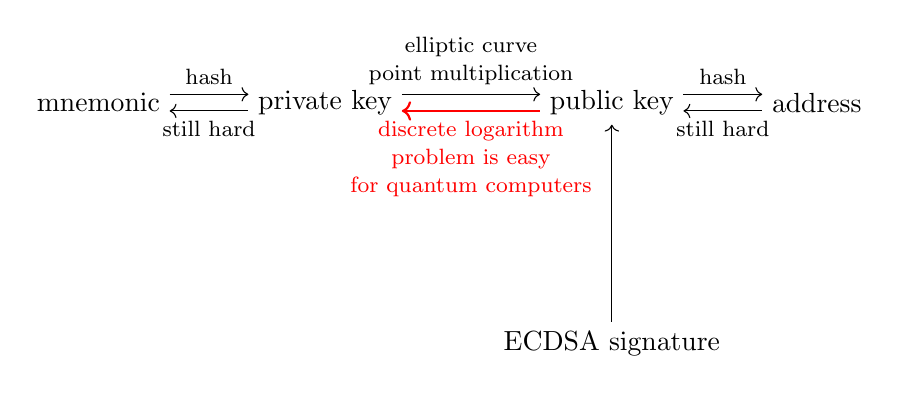
\begin{tikzpicture}

  \def\myoffset{0.3em}
  
  \node (mnemonic) {mnemonic};
  \node (privkey) [right=of mnemonic] {private key};
  \node (pubkey) [right=5em of privkey] {public key};
  \node (address) [right=of pubkey] {address};
  \node (signature) [below=2.5cm of pubkey] {ECDSA signature};

  \draw[->] ([yshift=\myoffset]mnemonic.east) -- ([yshift=\myoffset]privkey.west) node[midway, above, font=\footnotesize] {hash};
  \draw[->] ([yshift=\myoffset]privkey.east) -- ([yshift=\myoffset]pubkey.west) node[midway, above, font=\footnotesize] {\shortstack{elliptic curve \\ point multiplication}};
  \draw[->] ([yshift=\myoffset]pubkey.east) -- ([yshift=\myoffset]address.west) node[midway, above, font=\footnotesize] {hash};

  \draw[<-] ([yshift=-\myoffset]mnemonic.east) -- ([yshift=-\myoffset]privkey.west) node[midway, below, font=\footnotesize] {still hard};
  \draw[<-, thick, draw=red] ([yshift=-\myoffset]privkey.east) -- ([yshift=-\myoffset]pubkey.west) node[midway, below, font=\footnotesize, text=red] {\shortstack{discrete logarithm \\ problem is easy \\ for quantum computers}};
  \draw[<-] ([yshift=-\myoffset]pubkey.east) -- ([yshift=-\myoffset]address.west) node[midway, below, font=\footnotesize] {still hard};

  \draw[<-] (pubkey.south) -- (signature.north);

\end{tikzpicture}

\end{frame}

\begin{frame}[fragile]{Bitcoin price impact}
\newcommand{\centerx}{\dimexpr(\paperwidth - 17cm)/2}
\begin{textblock*}{17cm}(\centerx,1.5cm)
\centering
\includegraphics[trim={6cm 0 11.4cm 8.7cm},clip,scale=0.75]{forbes-bitcoin-news.pdf} % left bottom right top
\end{textblock*}
\end{frame}

\begin{frame}[fragile]{Bitcoin case}

In Bitcoin transactions, public keys can be exposed.

Early P2PK (pay to public key) transactions directly
 include the public key in the output part. Roughly 10\%
 of all Bitcoin, including those believed to belong to
 Satoshi Nakamoto, fall into this category.
 Recent P2TR (Taproot) transactions also expose public keys.

P2PKH (pay to public key hash) transactions hide
 the public key until the coins are spent. At that point,
 all unspent tokens associated with the same address become 
 vulnerable. The common Bitcoin practice of avoiding address
 can reduce public key exposure. Later P2WPKH (SegWit P2PKH),
 P2SH (pay to script hash) and P2WSH (SegWit P2SH) transactions
 may expose public keys when spent, too.
 
Public keys can also be revealed in mempool transactions
 before they are included in a block.

\end{frame}

\begin{frame}[fragile]{PQC (Post-Quantum Cryptography)}

Cryptography relies on hard problems. For example, RSA is based
 on the assumption that factoring the product of two large primes
 is hard. For over 2,000 years, no efficient method for factoring
 large numbers has been discovered, so RSA has been trusted.
 But quantum computers break this assumption. We need problems
 that are hard even for quantum machines.

Algorithms based on lattice, code theory, hash, multivariate and
 supersingular elliptic curve isogeny are being proposed as
 quantum-resistant solutions. In 2022, after a 6-year competition,
 NIST selected 4 primary algorithms for standardization and
 continues to evaluate new candidates.

{\scriptsize\selectfont
for encryption: (lattice-based) CRYSTALS-Kyber (ML-KEM), (new in 2025, code-based) HQC\\
for signature: (lattice-based) CRYSTALS-Dilithium (ML-DSA), Sphincs+ (SLH-DSA),\\
\vspace{-0.5\baselineskip}(hash-based) FALCON (FN-DSA)}

KpqC also finalized 4 PQC algorithms in 2025.
\end{frame}

\begin{frame}[fragile]{}

In 2022, an isogeny-based candidate, SIKE, relying
 on the SIDH assumption was broken and removed from the NIST selection.
\vspace{6.5cm}

\newcommand{\centerx}{\dimexpr(\paperwidth - 17cm)/2}
\begin{textblock*}{17cm}(\centerx,2.2cm)
\centering
\includegraphics[page=15,trim={0 0 0 0},clip,scale=0.75]{2023-04-Eurocrypt.pdf} % left bottom right top
\end{textblock*}
\end{frame}

\begin{frame}[fragile]{Blockchain and PQC}

Algorand, one of the few early adopters of PQC, has used
 the FALCON signature scheme since 2022. However, PQC tend to
 have larger key size and slower computation, which increase
 block size and verification time. This makes blockchains
 hesitant to adopt them.

Another concern is the relatively short history of these
 cryptographic assumptions. For comparison: factoring over 2,000 years,
 elliptic curves for 300 years (EC-DLP for 40 years),
 collision-resistant hashes for 50 years, and
 groups of unknown order for 20 years.

As a result, the idea of \emph{cryptographic agility}, designing
 systems that can easily switch cryptographic primitives,
 is gaining traction.

\end{frame}

\begin{frame}[fragile]{}
\newcommand{\centerx}{\dimexpr(\paperwidth - 17cm)/2}
\begin{textblock*}{17cm}(\centerx,1cm)
\centering
\includegraphics[trim={4cm 0 12cm 3.2cm},clip,scale=0.75]{solana-winternitz-vault.pdf} % left bottom right top
\end{textblock*}
\end{frame}

\begin{frame}[fragile]{Solana news}

A developer built a quantum-safe vault (token management smart contract)
 on Solana. Commands must be signed using hash-based signatures,
 secure against quantum computers.
 Solana native signature scheme is vulnerable
 to quantum computers, and it directly uses public keys as addresse
 without hashing. This smart contract approach adds quantum resistance
 without changing the protocol, and can apply to other blockchains, too.

\end{frame}

\begin{frame}[fragile]{}

A developer proposed a Bitcoin hard fork called
 the Quantum-Resistant Address Migration Protocol (QRAMP).
 The proposal requires users to move funds to
 Quantum-Resistant addresses secured by quantum-safe signatures.
 After a set deadline, transactions using legacy signatures
 would be rejected.
\vspace{5cm}

\newcommand{\centerx}{\dimexpr(\paperwidth - 17cm)/2}
\begin{textblock*}{17cm}(\centerx,3.6cm)
\centering
\includegraphics[trim={0 6cm 0 11cm},clip,scale=0.5]{bitcoin-qramp.pdf} % left bottom right top
\end{textblock*}
\end{frame}

\begin{frame}[fragile]{Ethereum case}

Ethereum account abstraction (AA), including EIP-4337, EIP-7702
 in upcoming Pectra hard fork and EIP-7701 in future, brings
 smart contract capabilities to regular accounts. One key benefit
 is support for new authentication methods such as 2FA and PQC.

Ethereum has other components that are also vulnerable to
 quantum attacks. See purple items in Vitalik roadmap.
\begin{itemize}
  \item ECDSA signatures in transaction
  \item BLS signatures in consensus
  \item KZG commitments in blob
  \item Bandersnatch curve (tentative) in Verkle \\ tree
\end{itemize}
\vspace{1.4cm}

\begin{textblock*}{3cm}(8.2cm,5cm)
\centering
\includegraphics[trim={0 0 0 0},clip,scale=0.1]{vitalik-roadmap.jpeg} % left bottom right top
\end{textblock*}

\begin{textblock*}{5cm}(2.5cm,6.9cm)
\centering
\includegraphics[trim={0 10cm 0 2cm},clip,scale=0.25]{eprint-2025-055.pdf} % left bottom right top
\end{textblock*}
\end{frame}

\begin{frame}[fragile]{}

Vitalik proposed an emergency hard fork in case
 quantum computers suddenly appear. The idea is
 to first roll back clearly compromised blocks and
 disable legacy transactions. Accounts can migrate to
 a quantum-proof state by submitting a new type
 of transaction that includes a quantum-resistant STARK
 zero-knowledge proof showing users know the mnemonic
 linked to their public key.
\vspace{5cm}

\newcommand{\centerx}{\dimexpr(\paperwidth - 17cm)/2}
\begin{textblock*}{17cm}(\centerx,4cm)
\centering
\includegraphics[trim={0 320cm 3.6cm 0cm},clip,scale=0.25]{vitalik-quantum-emergency.pdf} % left bottom right top
\end{textblock*}
\end{frame}

\begin{frame}[fragile]{}
\newcommand{\centerx}{\dimexpr(\paperwidth - 17cm)/2}
\begin{textblock*}{17cm}(\centerx,0.5cm)
\centering
\includegraphics[trim={0.5cm 8cm 0.5cm 9cm},clip,scale=0.6]{satoshi-post.pdf} % left bottom right top
\end{textblock*}

\begin{textblock*}{11cm}(1cm,8.5cm)
{\tiny Hash collision asks whether it’s possible to find or create
 two different inputs with the same hash output.
 If possible, it could rewrite past\\
 blocks linked by hash values.
 While there have been real-world attacks on hash functions
 due to unexpected weaknesses, but it's believed\\
 \vspace{-0.7\baselineskip}that quantum computers
 won't break collision resistance
 ($O(a^{\sfrac{n}{2}}) \longrightarrow O(a^{\sfrac{n}{3}})$
 by Brassard–Høyer–Tapp algorithm).}
\end{textblock*}

\end{frame}

\end{document}
